\chapter{Background}\label{ch:background}

To establish a clear foundation for the concepts and definitions introduced throughout this thesis, we provide a fundamental overview of the key topics relevant to this research. This includes an introduction to \ac{RTS}, \acf{IPC}, and synchronization techniques, with a particular focus on wait-free synchronization. Additionally, we examine the Rust programming language, as it serves as the primary development environment for this study. Furthermore, we explore existing synchronization methods in \ac{RTS} to contextualize the motivation and contributions of this work.

\section{Real-Time Systems}\label{sec:real-time}

In \ac{RTS} the correctness of the system does not only depend on the logical results of computations, but also on timing constraints. These systems can be classified into \ac{HRTS} or \ac{SRTS}. \ac{HRTS} have strict timing constraints, and missing a constraint is considered a system failure and may lead to a catastrophic desaster. The sysetem must guarantee that every timing constraint has to be met. An use case would be industrial automation where all the machines and robotic modules have to communicate with each other as quick as possible to ensure no blockage of the manufacturing line. \cite{HardSoftRealTime}

On the other hand, \ac{SRTS} try to stick to the timing constraints as much as possible, but missing some timing constraints is not considered a system failure. Infrastructure wise \ac{SRTS} are similar to \ac{HRTS}, since it is still considered important to meet these timing constraints. An example would be a multimedia system where it would be considered fine if sometimes frames are dropped to guarantee the video stream. \cite{HardSoftRealTime}

Sometimes these two systems appear in combination, where some functions have hard real-time constraints and some have soft real-time constraints. Krishna K. gives a good example in his paper where he describes that for the apollo 11 mission some components for the landing processes had soft real-time behavior and the rest still functioned with hard real-time constraints. \cite{HardSoftRealTime}

Since the workfield of this thesis is within \ac{HRTS}, the term \ac{RTS} will be used synonymously with the terminology \ac{HRTS}.

\section{Inter-Process Communication}\label{sec:ipc}

Now the processes used in a \ac{RTS} also have to share information with each other so the system can function. So some kind of \ac{IPC} is needed. \ac{IPC} allows processes to share information with each other using different kind of methods. We will mainly focus on one method explained later. In general \ac{IPC} is needed in all computing systems, because processes often need to work together (e.g. a producer process passes data to a consumer process). Lets take the brake-by-wire technology as example. Brake-by-wire is a technology for driverless cars where some mechanical and hydraulic components from the braking systems are replaced by wires to transmit braking signals, since there is no driver anymore to press on the braking pedal \cite{BrakeByWire}. This of course requires different processes to share information together. In the context of this thesis this kind of communication requires strict timing constraints as stated as before, since any kind of delay or blockage would lead to fatal consequences. \cite{IPC,IPCMechanisms}

To achieve \ac{IPC} different kind of mechanisms are used. The focus for this work lies on shared memory, so that is also the mechanism we will look into. 

\subsection{Shared Memory}\label{subsec:shared-memory}

To achieve any kind of information sharing between processes, these processes will need to have access to the same data regularly. With a shared memory segment, multiple processes can have access to the same memory location. So all processes which are part of the \ac{IPC} can read and write to this common memory space avoiding unnecessary data copys. With that processes exchange information by directly manipulating memory. This kind of \ac{IPC} is particular useful for real-time applications, which handle large volumes of data or are required to quickly transfer data between sensors and control tasks. What is also important to know is that the section of the code, that programs these data accesses by different processes is called critical section. \cite{IPCMechanisms,SharedMemory,SharedMemoryMessagePassing,criticalSectionMutex}

The problem with this is that the system somehow has to manage how the processes access the shared memory segment. This is mostly done by using different kind of synchronization techniques. Without any synchronization mechanism race conditions or inconsistent data can occur. \cite{IPCMechanisms, SharedMemory}

\section{Synchronization}\label{sec:synchronization}

So as we see, synchronization is a crucial part of \ac{IPC} in \ac{RTS}, especially when processes communicate via shared memory. Communication through shared memory always has a risk of race conditions (when multiple processes acces the same data and cause unexpected behaviour) and data inconsistency if the processes are not properly synchronized. Tratitional synchronization techniques ensure mutual exclusion (only one process at a time uses shared resource) thus avoiding race conditions and ensuring data consistency. Race conditions happen when for example two processes write to the same resource. Lets take a single counter instance with value 17 as a shared resource in a shared memory region. If one has process p1 and preocess p2 that increment the number we would think that the end result is 19. But what could happen is that p1 reads the value 17 and then p2 reads the value 17. Now internally both processes increment that number to 18 and both processes would write 18 to that shared resource. To understand this example more in detail \cref{fig:race-condition} visualizes a race condition with threads. The difference between processes and threads is just, that threads are part of a process which can perform multiple tasks simultaneously within that process \cite{DiffProcessThread}. So the concept shown in \cref{fig:race-condition} can be used for multiple processes too.

\begin{figure}[h!]
   \centering
   \captionsetup{justification=centering}
   \caption{Race condition between two threads, which write to the same shared variable \cite{Race-Condition}.}
   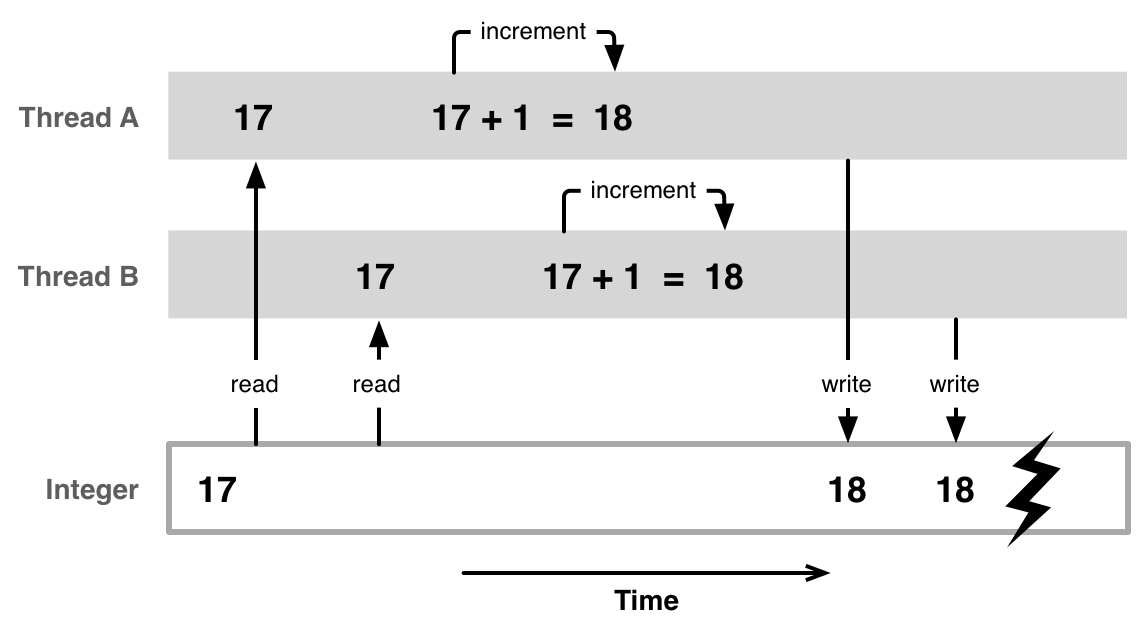
\includegraphics[width=115mm]{images/race-condition.png}
   \label{fig:race-condition}
\end{figure}

\subsection{Mutual Exclusion}\label{subsec:mutual-exclusion}

As discussed mutual exclusion does only allow one process or thread to access the shared resource at a time. This approach inherently relys on blocking some processes, which can lead to several issues, including deadlocks, process starvation, priority inversion, and increased response times. While explaining some of these problems, this paper will also give an superficial explanation on some non wait-free Sysnchronisation techniques. \cite{brandenburg2019multiprocessorrealtimelockingprotocols}

\subsubsection{Deadlock}\label{subsubsec:deadlock}



\subsubsection{Process Starvation}\label{subsubsec:process-starvation}



\subsubsection{Priority Inversion}\label{subsubsec:priority-inversion}

\section{Wait-Free Synchronization}\label{sec:wait-free}

\section{Lock-Free Synchronization}\label{sec:lock-free}

\section{Rust Programming Language}\label{sec:rust}

\section{State of the Art}\label{sec:state-of-the-art}